\chapter{Sicherheit}
\label{chap:Sicherheit}

\section{Halbwertschicht (Abschirmung)}
\label{sec:Halbwertschicht }
Wie im vor Abschnitt über die Strahlungstheorie diskutiert wurde, hängt die Eindringtiefe für eine gegebene Photonenenergie von der Materialdichte (Atomstruktur) ab. Je mehr subatomare Teilchen in einem Material vorliegen (höhere Z-Zahl), desto größer ist die Wahrscheinlichkeit, dass Wechselwirkungen auftreten und die Strahlung ihre Energie verliert. Je dichter ein Material ist, desto geringer ist daher die Eindringtiefe der Strahlung. Materialien wie abgereichertes Uran, Wolfram und Blei haben hohe Z-Zahlen und sind daher sehr wirksam bei der Abschirmung von Strahlung. Beton ist nicht so wirksam in der Abschirmung von Strahlung, aber es ist ein sehr gebräuchliches Baumaterial und wird daher häufig bei der Konstruktion von Strahlungsgewölben verwendet.\\
Da unterschiedliche Materialien die Strahlung in unterschiedlichem Maße abschwächen, wurde ein praktisches Verfahren zum Vergleichen der Abschirmungsleistung von Materialien benötigt. Die Halbwertschicht (HVL (Sehen das Bild\ \ref{fig:Half-Value-Layer})) wird üblicherweise für diesen Zweck verwendet und um zu bestimmen, welche Dicke eines gegebenen Materials notwendig ist, um die Belichtungsrate von einer Quelle auf ein bestimmtes Niveau zu reduzieren. Irgendwann im Material gibt es ein Niveau, bei dem die Strahlungsintensität die Hälfte derjenigen an der Oberfläche des Materials wird. Diese Tiefe wird als Halbwertschicht für dieses Material bezeichnet. Eine andere Betrachtungsweise ist, dass die HVL die Menge an Material ist, die notwendig ist, um die Belichtungsrate von einer Quelle auf die Hälfte ihres nicht abgeschirmten Werts zu reduzieren.\\
Manchmal ist die Abschirmung als eine Anzahl von HVL spezifiziert. Wenn zum Beispiel eine Gammaquelle 369 R / h an einem Fuß erzeugt und eine vier HVL-Abschirmung um sie herum angeordnet ist, würde die Intensität auf 23,0 R / h reduziert werden.

Jedes Material hat seine eigene spezifische HVL-Dicke. Das HVL-Material ist nicht nur abhängig, sondern auch strahlungsenergieabhängig. Dies bedeutet, dass sich für ein gegebenes Material, wenn sich die Strahlungsenergie ändert, sich auch der Punkt ändert, an dem die Intensität auf die Hälfte ihres ursprünglichen Werts abnimmt. Im Folgenden sind einige HVL-Werte für verschiedene Materialien aufgeführt, die üblicherweise in der industriellen Radiographie verwendet werden. Wie aus der Überprüfung der Werte ersichtlich ist, steigt mit steigender Energie der Strahlung auch der HVL-Wert (Sehen das Bild\ref{fig:halbwertszeit}).

\section{Strahlenbelastung kontrollieren}
\label{sec:Strahlenbelastung }
Wenn man mit Strahlung arbeitet, gibt es zwei Arten der Exposition: akute und chronische. Eine akute Exposition ist eine einmalige, versehentliche Exposition gegenüber einer hohen Strahlungsdosis während eines kurzen Zeitraums. Eine akute Exposition hat das Potenzial, sowohl nicht-stochastische als auch stochastische Effekte zu erzeugen. Chronische Exposition, die manchmal auch als "kontinuierliche Exposition" bezeichnet wird, ist eine langfristige Überexposition auf niedrigem Niveau. Eine chronische Exposition kann zu stochastischen Auswirkungen auf die Gesundheit führen und ist wahrscheinlich auf unsachgemäße oder unzureichende Schutzmaßnahmen zurückzuführen.\\
Die drei grundlegenden Möglichkeiten zur Kontrolle der Exposition gegenüber schädlicher Strahlung sind:\\
1) Begrenzung der Zeit in der Nähe einer Strahlungsquelle\\
2) Erhöhung der Entfernung von der Quelle\\
3) Mit einer Abschirmung, um das Strahlungsniveau zu stoppen oder zu reduzieren\\
\begin{figure}[htb]
  \centering  
  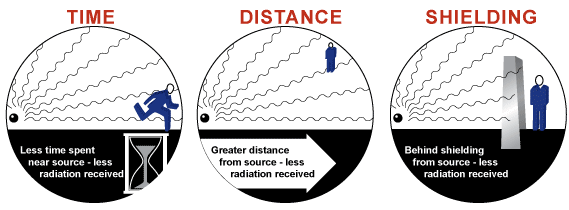
\includegraphics[scale=0.5]{img/TimeDistShield.png}
  \caption{Time Dist Shield}
  \label{fig:TimeDistShield}
\end{figure}\\
 Quelle: \url{https://www.nde-ed.org/index_flash.htm}
\subsection{Zeit}
Die Strahlungsdosis ist direkt proportional zu der Zeit, die in der Strahlung verbracht wird. Daher sollte sich eine Person nicht länger als nötig in der Nähe einer Strahlungsquelle aufhalten. Wenn ein Vermessungsgerät 4 mR / h an einem bestimmten Ort liest, wird eine Gesamtdosis von 4mR erhalten, wenn eine Person für eine Stunde an diesem Ort verbleibt. In einer zweistündigen Zeitspanne würde eine Dosis von 8 mR erhalten werden. Die folgende Gleichung kann verwendet werden, um eine einfache Berechnung durchzuführen, um die Dosis zu bestimmen, die in einem Strahlungsgebiet empfangen wird oder wurde.\\
Dose = Dose Rate x Time \\
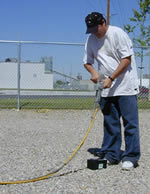
\includegraphics[scale=0.7]{img/timeDist.jpg}\\
Quelle: \url{https://www.nde-ed.org/index_flash.htm}\\
Bei Verwendung einer Gammakamera ist es wichtig, die Quelle von der abgeschirmten Kamera so schnell wie möglich zum Kollimator zu bringen, um die Expositionszeit der ungeschirmten Quelle zu begrenzen. Vorrichtungen, die Strahlung in einigen Richtungen abschirmen, aber in einer oder mehreren anderen Richtungen passieren können, sind als Kollimatoren bekannt. Dies wird in den Bildern am Ende dieser Seite veranschaulicht.
\subsubsection{Beispielrechnungen 1}
Ein Techniker befindet sich in einem Bereich für 10 Minuten und der Messwert auf dem Vermessungsmesser beträgt 5 mR / h. Welche Strahlendosis erhält der Techniker?\\
5mR/h / 60 min./h = 0.0833 mR/min.\\
0.0833 mR/min. x 10 min = 0.833 mR  total dose.\\

\subsubsection{Beispielrechnungen 2}
Ein Techniker möchte unter Berücksichtigung der oben genannten Bedingungen nicht mehr als eine Dosis von 1,0 mR erhalten. Wie lange kann der Techniker maximal in der Gegend bleiben?\\
1.0 mR / 0.0833 mR/min. = 12 min \\
Die berechneten Dosierungen wären Annäherungen. Die tatsächlichen Dosierungen können aufgrund von Streuung und anderen Überlegungen variieren. Die TLD oder das Film-Badge sollte verwendet werden, um die von einer Person erhaltene Dosis zu bestimmen.
\subsection{Entfernung}
Die zunehmende Entfernung von der Strahlungsquelle verringert die Menge der empfangenen Strahlung. Wenn Strahlung von der Quelle ausgeht, breitet sie sich aus und wird weniger intensiv.\\
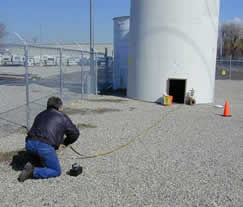
\includegraphics[scale=0.5]{img/distance.jpg}\\
Quelle: \url{https://www.nde-ed.org/index_flash.htm}\\
Dies ist vergleichbar mit dem Stehen in der Nähe eines Feuers. Je näher eine Person dem Feuer steht, desto intensiver fühlt sich die Hitze vom Feuer an. Dieses Phänomen kann durch eine Gleichung ausgedrückt werden, die als das umgekehrte quadratische Gesetz bekannt ist, das besagt, dass, wenn sich die Strahlung von der Quelle ausbreitet, die Dosierung umgekehrt zum Quadrat der Entfernung abnimmt.\\
Berechnung der Intensität mit dem inversen Quadratgesetz: \\

\( \frac {I1}  {I2} = \frac {D2^2} { D1^2} \) \\
\\
I1 = Intensität 1 bei D1 \\
I2 = Intensität 2 bei D2 \\
D1 = Entfernung 1 von der Quelle\\
D2 = Entfernung 2 von der Quelle\\

\subsubsection{Beispielrechnungen 1}
Die Strahlungsintensität beträgt 530 U / h bei 5 Fuß Entfernung von einer Quelle. 
Wie groß ist die Intensität der Strahlung bei 10 Fuß?
Überarbeiten Sie die Gleichung, um die Intensität in Entfernung 2 zu lösen:\\
\( I2 = I1*\frac{D1^2} { D2^2} \) \\
Stecken Sie die bekannten Werte ein\\
\( I2 = 530R/h * \frac{(5ft)^2} {(10ft)^2} \) \\

Löse für I2= 132.5 R/h \\
In diesem Fall wurde die Entfernung verdoppelt und die Intensität an diesem Punkt hat sich um den Faktor vier verringert.

\subsubsection{Beispielrechnungen 2}
Eine Quelle erzeugt eine Intensität von 456 R / h bei einem Fuß von der Quelle. Wie groß wäre der Abstand in Fuß zu den 100, 5 und 2 mR / h Grenzen.\\
Konvertiere R / Stunde in mR / Stunde\\
456R/h * 1000 = 456,000 mR/h\\
\big (\ D2 = $\sqrt[\leftroot{3}\uproot{3}]{\tfrac{I1*D1^2}{I2}}$  \big) -----> \Big(
\ D2 = $\sqrt[\leftroot{3}\uproot{3}]{\tfrac{456,000 mR/h * (1ft)^2}{100 mR/h}}$ \Big) ---> \Bigg(D2= 67.5 \Bigg) 
\subsection{Abschirmung}
Der dritte Weg, die Strahlenexposition zu reduzieren, besteht darin, etwas zwischen dem Radiographen und der Strahlungsquelle zu platzieren. Im Allgemeinen gilt, je dichter das Material ist, desto mehr Abschirmung wird es bereitstellen. Die wirksamste Abschirmung wird durch Metall aus abgereichertem Uran erreicht. Es wird hauptsächlich in Gammastrahlenkameras wie der unten gezeigten verwendet.\\
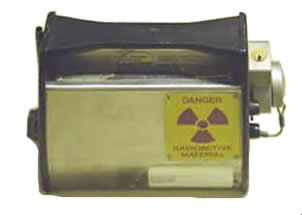
\includegraphics[scale=0.9]{img/cameraoutside.jpg}\\ 
 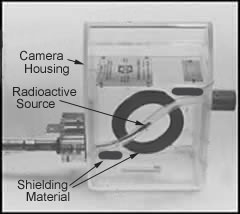
\includegraphics[scale=0.5]{img/camera_pigtail.jpg}\\
 Quelle: \url{https://www.nde-ed.org/index_flash.htm}\\
Der Kreis aus dunklem Material in der Plastik-Durchsichtskamera (unten rechts) wäre tatsächlich eine Kugel aus abgereichertem Uran in einer echten Gammastrahlenkamera. Abgereichertes Uran und andere Schwermetalle, wie Wolfram, sind sehr wirksam bei der Abschirmung von Strahlung, da ihre dicht gepackten Atome es der Strahlung schwer machen, sich durch das Material zu bewegen, ohne mit den Atomen in Wechselwirkung zu treten. Blei und Beton sind die am häufigsten verwendeten Strahlenschutzmaterialien, hauptsächlich weil sie einfach zu verarbeiten sind und leicht verfügbar sind. Beton wird häufig bei der Konstruktion von Strahlungsgewölben verwendet. Einige Gewölbe werden auch mit Bleifolien verkleidet, um die Strahlung auf ein akzeptables Maß von außen zu reduzieren.

\begin{figure}[htb]
\centering
  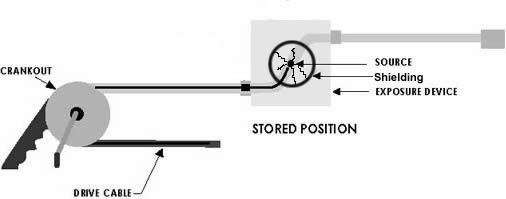
\includegraphics[scale=0.4]{img/Gamma1.jpg}\\
  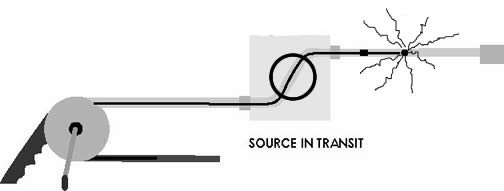
\includegraphics[scale=0.4]{img/Gamma2.jpg}\\
  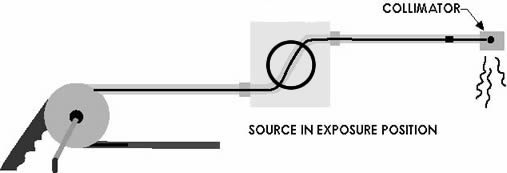
\includegraphics[scale=0.4]{img/Gamma3.jpg}\\
  \caption{Camera}
  \label{fig:Camera}
\end{figure}
Quelle: \url{https://www.nde-ed.org/index_flash.htm}
\section{Sicherheitskontrollen}
\label{kontrollen}
Da Röntgen- und Gammastrahlung von den menschlichen Sinnen nicht wahrgenommen werden können und der daraus resultierende Schaden für den Körper nicht unmittelbar ersichtlich ist, wird eine Vielzahl von Sicherheitskontrollen verwendet, um die Exposition zu begrenzen. Die zwei grundlegenden Arten von Strahlenschutzkontrollen, die für eine sichere Arbeitsumgebung verwendet werden, sind technische und administrative Kontrollen. Engineered Kontrollen umfassen Abschirmung, Verriegelungen, Alarme, Warnsignale und Materialeinschließung. Administrative Kontrollen umfassen Buchungen, Prozeduren, Dosimetrie und Schulungen.
\subsection{Engineered Kontrollen}
Engineered Kontrollen wie Abschirmung und Türverriegelungen werden benutzt, um die Strahlung in einem Kabinett oder in einem "Strahlungsgewölbe" zu enthalten.
Feste Abschirmungsmaterialien sind üblicherweise Beton und / oder Blei mit hoher Dichte. Türverriegelungen werden verwendet, um den Strom zu Röntgenstrahlen erzeugenden Geräten sofort zu unterbrechen, wenn eine Tür versehentlich geöffnet wird, wenn Röntgenstrahlen erzeugt werden. Warnlichter werden verwendet, um Arbeiter und die Öffentlichkeit darauf aufmerksam zu machen, dass Strahlung verwendet wird. Sensoren und Warnalarme werden oft verwendet, um zu signalisieren, dass eine vorbestimmte Menge an Strahlung vorhanden ist. Sicherheitskontrollen sollten niemals manipuliert oder umgangen werden.\\
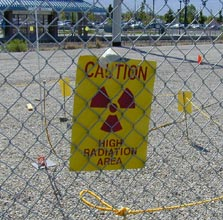
\includegraphics[scale=0.9]{img/safetyshild.jpg}\\
Wenn eine tragbare Radiographie durchgeführt wird, ist es meistens nicht praktikabel, Alarm- oder Warnlichter im Belichtungsbereich zu platzieren. Seile und Schilder werden verwendet, um den Zugang zu Strahlungsbereichen zu blockieren und die Öffentlichkeit auf das Vorhandensein von Strahlung aufmerksam zu machen. Gelegentlich verwenden Radiografen batteriebetriebene Blitzlichter, um die Öffentlichkeit auf das Vorhandensein von Strahlung aufmerksam zu machen. Tragbare oder temporäre Abschirmvorrichtungen können aus Materialien oder Geräten hergestellt werden, die sich im Bereich der Inspektion befinden. Zur vorübergehenden Abschirmung können Stahlbleche, Stahlträger oder andere Geräte verwendet werden. Es liegt in der Verantwortung des Radiografen, den Absorptionswert verschiedener Materialien zu kennen und zu verstehen. Weitere Informationen zu Absorptionswerten und Materialeigenschaften finden Sie im Röntgenbereich dieser Website.
\subsection{Verwaltungskontrollen}
Wie bereits erwähnt, ergänzen administrative Kontrollen die technischen Kontrollen. Diese Steuerelemente umfassen Buchungen, Prozeduren, Dosimetrie und Training. In der Regel ist es erforderlich, dass alle Bereiche, in denen röntgenstrahlerzeugende Geräte oder radioaktive Materialien enthalten sind, mit Schildern versehen sind, auf denen das Strahlungssymbol und ein Hinweis auf die Gefahren der Strahlung angebracht sind. Normale Betriebsverfahren und Notfallverfahren müssen ebenfalls vorbereitet und befolgt werden. In den USA schreibt das Bundesgesetz vor, dass jede Person, die wahrscheinlich mehr als 10\% eines jährlichen Arbeitsplatzgrenzwerts erhält, auf Strahlenbelastung überwacht wird. Diese Überwachung wird durch den Einsatz von Dosimetern erreicht, die im Abschnitt Strahlungssicherheitsausrüstung dieses Materials behandelt werden. Eine gute Schulung mit begleitender Dokumentation ist auch eine sehr wichtige administrative Kontrolle.\\
Quelle: \url{https://www.nde-ed.org/index_flash.htm}

\subsection{Strahlenschutzbereiche}
Strahlenschutzgebiete werden bei Tätigkeiten eingerichtet, für die eine Genehmigung nach den nationalen Strahlenschutzgesetzen erforderlich ist. Je nach Strahlenexposition wird zwischen Überwachungsbereichen, Kontrollbereich und Sperrbereich hinsichtlich der externen und internen Strahlenexposition unterschieden. Überall dort, wo EU-Vorschriften gelten, gelten folgende Werte:\\

{\rowcolors{3}{yellow}{green}
\begin{tabular}{ |p{2.5cm}|p{4cm}|p{4cm}|  }
\hline
\multicolumn{3}{|c|}{Strahlenschutzbereiche} \\
\hline
Isotop Quelle& Sperrbereich &Kontrollbereich \\
\hline
Iridium192 &1.6 $\sqrt{Aktivität}$&14 $\sqrt{Aktivität}$\\
\hline
Cobalt 60&2.6 $\sqrt{Aktivität}$&23 $\sqrt{Aktivität}$ \\
\hline
Cesium 137&1.3 $\sqrt{Aktivität}$& 11.5 $\sqrt{Aktivität}$\\
\hline
Ytterbium169&0.8 $\sqrt{Aktivität}$&7 $\sqrt{Aktivität}$ \\
\hline
\end{tabular} \\
Quelle: Ghiassi-Nejad, M., Katouzi, M. (2004).
Hefazat dar barbare aschaeh (Schutz gegen radioaktive Strahlung). 2. Band. 8. Auflage.
Teheran: Iranische Nationalbibliothek.\\
\subsubsection{Überwachungsbereich}
Überwachungsbereiche sind die Bereiche, in denen Personen eine höhere effektive Dosis als 1 mSv oder höhere Organdosen als 15 mSv für die Augenlinse oder 50 mSv für die Haut, die Hände, die Unterarme, die Füße und Knöchel im Kalenderjahr erhalten können. Oft wird das gesamte Betriebsgelände als Überwachungsbereich betrachtet und (zum Beispiel bei Kernkraftwerken) durch einen Zaun oder ähnliche Maßnahmen vom allgemeinen Staatsgebiet abgetrennt.
\subsubsection{Kontrollbereich}
Der Kontrollbereich ist meist vom Überwachungsbereich umschlossen. In ihm können Personen eine effektive Dosis von mehr als 6 mSv pro Kalenderjahr oder höhere Organdosen als 45 mSv pro Kalenderjahr für die Augenlinse oder 150 mSv pro Kalenderjahr für die Haut, die Hände, die Unterarme, die Füße und Knöchel erhalten. Kontrollbereiche müssen abgegrenzt und deutlich sichtbar gekennzeichnet sein. Ein Kontrollbereich darf nur zur Durchführung oder Aufrechterhaltung der vorgesehenen Betriebsvorgänge betreten werden. Besucher haben nur mit behördlicher Erlaubnis Zutritt. Bei Personen, die sich im Kontrollbereich aufhalten, müssen die Körperdosen bestimmt werden – üblicherweise mit einem amtlichen Dosimeter. Vor dem erstmaligen Zutritt und dann mindestens jährlich muss eine Unterweisung insbesondere über die anzuwendenden Strahlenschutzmaßnahmen durchgeführt werden.

\subsubsection{Sperrbereich}
Sperrbereiche sind Bereiche innerhalb eines Kontrollbereichs, in denen die Ortsdosisleistung höher als 3 mSv pro Stunde sein kann. Personen darf der Aufenthalt in einem Sperrbereich nur erlaubt werden, wenn sie unter der Aufsicht einer beauftragten fachkundigen Person zur Durchführung vorgesehener Betriebsvorgänge oder aus zwingendem Grund tätig werden müssen. Sperrbereiche sind abzugrenzen und deutlich sichtbar zu kennzeichnen.
Der Zutritt zu Strahlenschutzbereichen ist nicht frei. Einschränkungen finden sich z. B.in der deutschen StrlSchV (§ 37 Zutritt zu Strahlenschutzbereichen) für Überwachungs-, Kontroll- und Sperrbereiche.
Für alle übrigen Bereiche eines Betriebes, die nicht Strahlenschutzbereiche sind, gilt der Grenzwert für das allgemeine Staatsgebiet für die Ortsdosisleistung von 1 mSv pro Jahr.
\begin{figure}[htb]
  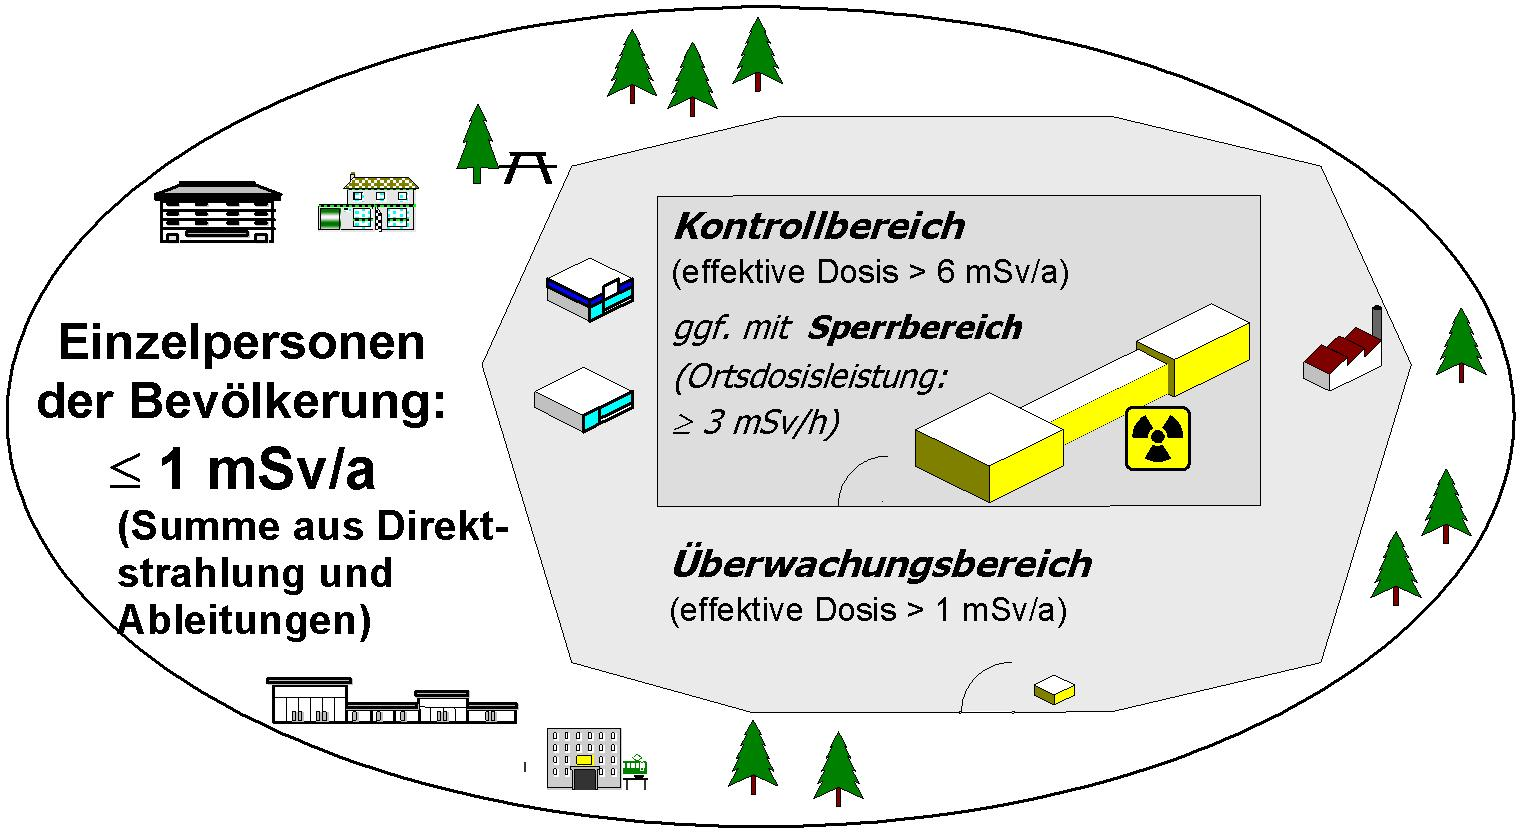
\includegraphics[scale=0.3]{img/Strahlenschutzbereiche.jpg}\\
  \caption{Strahlenschutzbereiche}
  \label{fig:Strahlenschutzbereiche}
  Quelle: \url{https://de.wikipedia.org/wiki/Strahlenschutzbereich}\\
\end{figure}

\section{Verantwortlichkeiten}
Der sichere Umgang mit der Strahlung liegt in der Verantwortung aller, die an der Verwendung und Verwaltung von strahlungserzeugenden Geräten und Materialien beteiligt sind. Abhängig von der Größe der Organisation können bestimmte Verantwortlichkeiten verschiedenen Personen und / oder Ausschüssen zugewiesen werden.
\subsection{Strahlenschutzbeauftragter \\ Radiation Safety Officer (RSO)/ Health Physics Safety (HPS)}
\label{sec:strahlenschutzbeauftragter}

Alle Organisationen, die zur Verwendung ionisierender Strahlung zugelassen sind, müssen über einen Strahlenschutzbeauftragten (RSO/HPS) verfügen. Der RSO/HPS ist die vom Unternehmen autorisierte Person, die als Ansprechpartner für alle Aktivitäten dient, die im Rahmen der Genehmigung durchgeführt werden. Der RSO/HPS stellt sicher, dass Strahlenschutzaktivitäten in Übereinstimmung mit genehmigten Verfahren und regulatorischen Anforderungen durchgeführt werden. Einige der gemeinsamen Verantwortlichkeiten für den RSO sind:\\
\begin{figure}
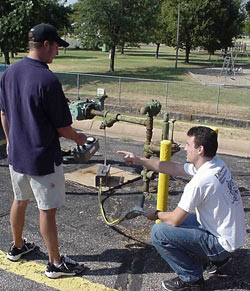
\includegraphics[scale=0.7]{img/rso.jpg}\\
Quelle: \url{https://www.nde-ed.org/index_flash.htm}
\end{figure}
\begin{enumerate}
  \item Sicherstellen, dass alle Personen, \\die Strahlengeräte verwenden, angemessen geschult     und beaufsichtigt werden.
  \item Sicherstellen, dass alle Personen, \\die das Gerät benutzen, formell zur Verwendung des Geräts autorisiert wurden.
  \item Sicherstellen, dass alle Regeln, \\Vorschriften und Verfahren für den sicheren Umgang mit  radioaktiven Quellen und Röntgensystemen eingehalten werden.
  \item Sicherstellen, dass geeignete Betriebs,Notfall- und ALARA-Verfahren \\entwickelt wurden und allen Systembenutzern zur Verfügung stehen.
  \item Sicherstellen, dass genaue Aufzeichnungen \\ über die Verwendung der Quellen und Geräte erhalten bleiben.
  \item Sicherstellen, dass die erforderlichen Strahlungsuntersuchungen und Dichtigkeitsprüfungen durchgeführt und dokumentiert werden.
  \item Sicherstellen, dass Systeme und Geräte vor unbefugtem Zugriff oder Entfernung geschützt sind.
\end{enumerate}
Die Mindestqualifikationen, Schulungen und Erfahrungen für RSOs für die industrielle Radiographie sind wie folgt: (1) Abschluss der Trainings- und Testanforderungen von Sec. 34.43 (a) von Teil 10 des Federal Code of Regulations, (2) 2000 Stunden praktische Erfahrung als qualifizierte Radiotechniker in industriellen radiographischen Operationen, und (3) Formale Ausbildung in der Einrichtung und Wartung eines Strahlenschutzprogramms.
\subsection{Strahlenschutzausschuss "Radiation Safety Committee" (RSC)}
Einige Organisationen haben möglicherweise einen Strahlenschutzausschuss (RSC), der den RSO/HPS unterstützt. Das RSC überwacht häufig die Richtlinien, Verfahren und Verantwortlichkeiten eines Strahlenschutzprogramms eines Unternehmens.
\subsection{Systembenutzer}
Die zur Verwendung des röntgenstrahlerzeugenden Systems oder der Gammaquellen autorisierten Personen sind dafür verantwortlich, dass :
\begin{enumerate}
\item Alle Regeln, Vorschriften und Verfahren zur sicheren Verwendung des Röntgensystems werden befolgt.
\item Eine genaue Aufzeichnung der Verwendung des Systems wird aufrechterhalten.
\item Alle Sicherheitsprobleme mit dem System werden dem RSO gemeldet und vor der weiteren Verwendung korrigiert.
\item Das System ist vor unbefugtem Zugriff oder Entfernung geschützt.
\end{enumerate}
\subsection{Verfahren}
Schriftliche Arbeitsanweisungen müssen entwickelt und jedem zur Verfügung gestellt werden, der mit Strahlenquellen oder röntgenstrahlenden Geräten arbeitet. Diese Verfahren müssen für die Ausrüstung und ihre Verwendung in einer bestimmten Anwendung spezifisch sein. Den Beschäftigten die Bedienungsanleitung des Geräteherstellers einfach zur Verfügung zu stellen, genügt dieser Anforderung nicht. Das Betriebsverfahren muss jederzeit befolgt werden, es sei denn, es liegt eine schriftliche Genehmigung des Strahlenschutzbeauftragten vor.
\subsubsection{Standardablauf}
Die Betriebsanweisungen müssen mindestens Anweisungen für Folgendes enthalten:
\begin{enumerate}
\item Angemessene Handhabung und Verwendung lizenzierter umschlossener Strahlenquellen und radiographischer Expositionsgeräte, so dass keine Person Strahlenexpositionen ausgesetzt ist, die über den festgelegten Expositionsgrenzwerten liegen.
\item Methoden und Anlässe für die Durchführung von Strahlungsuntersuchungen.
\item Methoden zur Kontrolle des Zugangs zu Radiographiebereichen.
\item Methoden und Anlässe zum Sichern und Sichern von Röntgengeräten, Transport- und Lagerbehältern und versiegelten Quellen.
\item Personalüberwachung und Einsatz von Personalüberwachungsgeräten.
\item Transport von versiegelten Quellen zu Feldstandorten, einschließlich Verpackung radiographischer Expositionsgeräte und Lagerbehälter in den Fahrzeugen, Plakatierung von Fahrzeugen bei Bedarf und Kontrolle der versiegelten Quellen während des Transports.
\item Überprüfung, Wartung und Funktionsfähigkeitsprüfung von Röntgengeräten, Vermessungsinstrumenten, Transportbehältern und Lagerbehältern.
\item Das Verfahren zur Identifizierung und Meldung von Mängeln und Nichteinhaltung.
\item Wartung von Aufzeichnungen.

\end{enumerate}

\subsubsection{Notfallmaßnahmen}
Es müssen auch Verfahren entwickelt werden, die die Mitarbeiter im Notfall leiten. Einige der Elemente, die abgedeckt werden könnten, sind:\\
\begin{enumerate}
\item Schritte, die sofort von dem Radiographiepersonal ergriffen werden müssen, wenn festgestellt wird, dass ein Taschendosimeter außerhalb der Skala liegt oder ein Alarmratenmesser unerwartet alarmiert.
\item Schritte zur Minimierung der Exposition von Personen im Falle eines Unfalls.
\item Das Verfahren zur Benachrichtigung der richtigen Personen im Falle eines Unfalls.
\item Wiederherstellungsprozedur für radioaktive Quellen, wenn der Lizenznehmer die Wiederherstellung durchführt.

\end{enumerate}
\subsection{Umfragetechnik}
Die Mehrheit der Überbelichtungen in der industriellen Radiographie ist das Ergebnis dessen, dass der Radiograf den Ort eines Gammastrahlers nicht kennt und keine geeignete Strahlungserhebung durchführt.
Expositionsgewölbe sind mit Warnleuchten und Sicherheitsverriegelungsschaltern ausgestattet, die eine Sicherheitsmarge für die Arbeiter bieten. Es muss gelegentlich eine Untersuchung durchgeführt werden, um sicherzustellen, dass in den Tresoren keine Strahlung austritt und dass die Sicherheitsvorrichtungen ordnungsgemäß funktionieren. Wenn jedoch eine Radiographie mit Gammastrahlern im Feld durchgeführt wird, muss sich der Röntgengeräteher stark auf Messungen mit einem Vermessungsmeter verlassen, da andere Sicherheitsvorrichtungen nicht üblich sind. Eine Reihe von Erhebungen muss durchgeführt werden, und einige der Ergebnisse dieser Erhebungen müssen dokumentiert werden, wenn mit Gammastrahlern im Feld transportiert und gearbeitet wird.
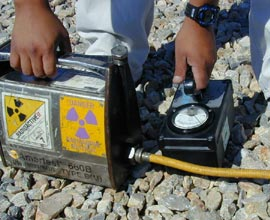
\includegraphics[scale=0.9]{img/cameraTest.jpg}\\
\subsubsection{Annäherung an das Belichtungsgerät}
Ein Techniker sollte sich gründlich mit dem Betrieb eines Vermessungsmessers auskennen, da der bestimmungsgemäße Gebrauch des Geräts unerlässlich ist. Bevor das Belichtungsgerät (Kamera) aus dem Speicher genommen wird, muss die Kalibrierung des Vermessungszählers überprüft und der Batteriestand überprüft werden. Wenn Sie sich dem Belichtungsgerät nähern, um es vom Lagerort zu entfernen, sollte das Vermessungsgerät griffbereit und betriebsbereit sein. Der Vermessungsmesser sollte neben dem Belichtungsgerät platziert werden, um zu überprüfen, ob die Quelle im Projektor enthalten ist, und um sicherzustellen, dass das Vermessungsgerät ordnungsgemäß funktioniert. Vermessungszählerstände sollten mit früheren Messungen verglichen und aufgezeichnet werden.
\subsubsection{Transport des Belichtungsgeräts}
Wenn das Belichtungsgerät transportiert wird, muss es sicher im Fahrzeug verstaut werden. Eine verschließbare Metallbox ist oft im Heck des Fahrzeugs verschraubt. Ein Überblick über die Überverpackung, die Außenseite des Fahrzeugs und den Fahrerraum wird dann durchgeführt und dokumentiert.
\subsubsection{Vorbereitung auf eine Exposition}
Auf der Baustelle wird der Expositionsbereich bewertet, Abstandsberechnungen für die Begrenzung der Sperrzonen und Seile und Schilder, die entsprechend platziert werden, durchgeführt. Sobald dies abgeschlossen ist, ist der Röntgentechniker bereit, das Belichtungsgerät aus seinem Ablagefach im Fahrzeug zu entfernen. Der Vermessungszähler sollte überwacht werden, wenn das Aufbewahrungsfach angefahren wird und wenn das Expositionsgerät aus dem Fach entfernt wird. Tägliche Sicherheitskontrollen sollten dann durchgeführt werden. Sobald diese Überprüfungen abgeschlossen sind, können der Röntgenassistent und der Assistent das Belichtungsgerät zum Expositionsort bewegen. Da die Kurbeln und Führungsrohre zur Vorbereitung der ersten Exposition angebracht sind, sollte das Vermessungsgerät überwacht werden. Bevor die Quelle freigelegt wird, sollte der Assistent den Bereich auf Personen überprüfen, die möglicherweise in den eingeschränkten Bereich eingedrungen sind, und sich dann außerhalb der Seilgrenze bewegen.
\subsubsection{Eine Belichtung erledigen}

Der Röntgentechniker sollte sich in der maximalen Entfernung von der Belichtungsvorrichtung befinden, die das Führungsrohr erlaubt, wenn er oder sie die Quelle schnell aus der Belichtungsvorrichtung herausritzt und einrastet. Wenn sich die Quelle aus dem Belichtungsgerät bewegt, wird der Vermessungsmesser auf ein sehr hohes Niveau ansteigen und sich dann verringern, sobald sich die Quelle innerhalb des Kollimators befindet. Während der Exposition wird der Assistent die festgelegte Grenze überwachen, um die vorhandenen Strahlungswerte zu bestimmen. Wenn der Vermessungsmesser anzeigt, dass die Werte höher als berechnet sind, muss die Grenze erweitert werden.
\subsubsection{Die Quelle zurückziehen}
Beim Zurückziehen der Quelle sehen die Röntgenphotographen einen Anstieg der Messwerte, wenn sich die Quelle aus dem Kollimator bewegt und in den Projektor zurückgezogen wird. Wenn sich die Quelle innerhalb des Belichtungsgeräts befindet, sollte sich der Röntgentechniker ihm nähern, während er den Vermessungsmesser überwacht. Wenn die Quelle ordnungsgemäß eingefahren ist, sollte bei Annäherung an das Belichtungsgerät keine Erhöhung des Messgeräts angezeigt werden. Das Belichtungsgerät sollte von allen Seiten beobachtet werden, wobei besonders auf die Vorderseite des Geräts zu achten ist. Die gesamte Länge des Führungsrohrs muss dann vermessen werden.

Dieser Vorgang wird für jede Belichtung wiederholt. Die Ergebnisse der Untersuchung müssen dokumentiert werden, wenn das Expositionsgerät zum Transport an das Fahrzeug zurückgegeben wird und wenn es an seinen Lagerort zurückgebracht wird.\\
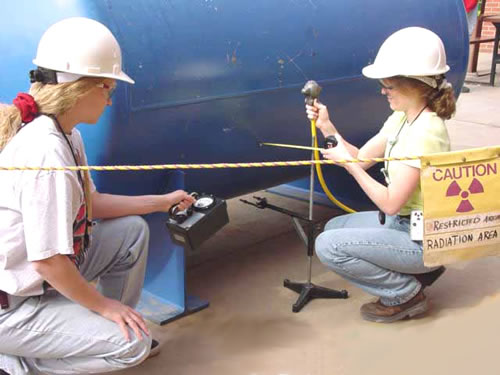
\includegraphics[scale=0.7]{img/isotope-radiography-pressure-vessel.jpg}\\
\subsection{Strahlungsdetektoren}
Instrumente zur Strahlungsmessung fallen in zwei große Kategorien:
\begin{itemize}
\item Messgeräte 
\item Persönliche Dosismessgeräte. 
\end{itemize}
\begin{figure}
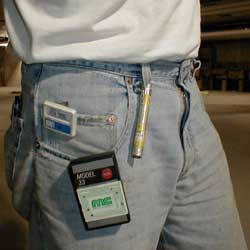
\includegraphics[scale=0.5]{img/strahlungsdetektor.jpg}\\
Quelle: \url{https://www.nde-ed.org/index_flash.htm}
\end{figure}
Frequenzmessgeräte messen die Rate, mit der die Belichtung empfangen wird 
(häufiger als Strahlungsintensität bezeichnet).
Vermessungszähler, akustische Alarme und Bereichsüberwachungsgeräte fallen in diese Kategorie. Diese Instrumente zeigen eine Strahlungsintensitätsablesung relativ zur Zeit, wie etwa R / h oder mR / h. Eine Analogie kann zwischen diesen Instrumenten und dem Tachometer eines Autos hergestellt werden, da beide Messeinheiten relativ zur Zeit sind.
Dosismessgeräte sind solche, die den Gesamtbetrag der während eines Messzeitraums erhaltenen Exposition messen. Die Dosimeter oder Dosimeter, die üblicherweise in der industriellen Radiographie verwendet werden, sind kleine Vorrichtungen, die dazu bestimmt sind, von einer Person getragen zu werden, um die von der Person empfangene Exposition zu messen. Eine Analogie kann zwischen diesen Instrumenten und dem Kilometerzähler eines Autos hergestellt werden, da beide akkumulierte Einheiten messen.

\subsection{Messgeräte}
Der Vermessungsmesser ist die wichtigste Ressource, die ein Röntgentechniker benötigt, um die Anwesenheit und Intensität der Strahlung zu bestimmen. Eine Überprüfung der Vorfall- und Überbelichtungsberichte zeigt, dass ein Großteil dieser Art von Ereignissen aufgetreten ist, wenn ein Techniker kein Vermessungsinstrument verwendet hat oder nicht verwendet hat.\\
Zur Messung der Strahlung im Feld stehen viele verschiedene Modelle von Vermessungszählern zur Verfügung. Sie alle bestehen im Wesentlichen aus einem Detektor und einer Ausleseanzeige. Analoge und digitale Anzeigen sind verfügbar. Die meisten Vermessungsmesser, die für die industrielle Radiographie verwendet werden, verwenden einen gasgefüllten Detektor.\\
\begin{figure}[htb]
  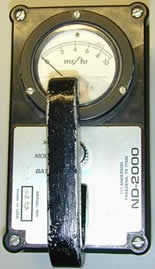
\includegraphics[scale=0.5]{img/radiometer.jpg}\\
  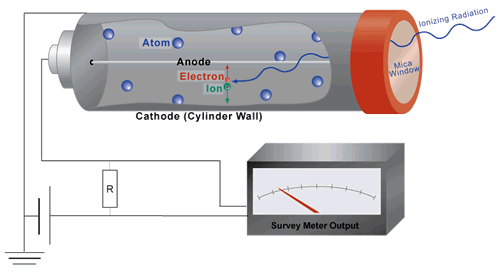
\includegraphics [scale=0.5]{img/radiometer_technik.png}
  \caption{Radiometer}
  \label{fig:radiometer}
  Quelle: \url{https://www.nde-ed.org/index_flash.htm}
\end{figure}
Gasgefüllte Detektoren bestehen aus einem gasgefüllten Zylinder mit zwei Elektroden. Manchmal wirkt der Zylinder selbst als eine Elektrode, und eine Nadel oder ein dünner straff gespannter Draht entlang der Achse des Zylinders wirkt als die andere Elektrode. Eine Spannung wird an die Vorrichtung angelegt, so dass die zentrale Nadel oder der Draht eine Anode (+ Ladung) wird und die andere Elektrode oder Zylinderwand die Kathode (- Ladung) wird. Das Gas wird ionisiert, sobald der Zähler in die Nähe von radioaktiven Substanzen gebracht wird. Das elektrische Feld, das durch die Potentialdifferenz zwischen der Anode und der Kathode erzeugt wird, bewirkt, dass sich die Elektronen jedes Ionenpaars zur Anode bewegen, während das positiv geladene Gasatom zur Kathode gezogen wird. Dies führt zu einem elektrischen Signal, das verstärkt wird, mit der Belichtung korreliert und als Wert angezeigt wird.\\
Abhängig von der zwischen der Anode und der Kathode angelegten Spannung kann der Detektor als eine Ionenkammer, ein Proportionalzähler oder ein Geiger-Müller (GM) -Detektor betrachtet werden. Jeder dieser Detektortypen hat seine Vor- und Nachteile. Eine kurze Zusammenfassung jedes dieser Detektoren folgt.
\subsubsection{Ionenkammerzähler}
Ionenkammern haben eine relativ niedrige Spannung zwischen der Anode und der Kathode, was zu einer Ansammlung von nur den Ladungen führt, die bei dem anfänglichen Ionisationsereignis erzeugt werden. Diese Art von Detektor erzeugt ein schwaches Ausgangssignal, das der Anzahl der Ionisationsereignisse entspricht. Höhere Energien und Strahlungsintensitäten erzeugen mehr Ionisierung, was zu einer stärkeren Ausgangsspannung führt.\\
Die Sammlung von nur primären Ionen liefert Informationen über die tatsächliche Strahlenbelastung (Energie und Intensität). Die Messgeräte benötigen jedoch eine empfindliche Elektronik, um das Signal zu verstärken, was sie ziemlich teuer und empfindlich macht. Der zusätzliche Aufwand und die erforderliche Sorgfalt sind gerechtfertigt, wenn genaue Strahlenexpositionsmessungen über einen Bereich von Strahlungsenergien durchgeführt werden müssen. Dies könnte notwendig sein, wenn die von einem Röntgengenerator erzeugte Bremsstrahlungsstrahlung gemessen wird. Ein Ionenkammer-Vermessungsmesser wird manchmal bei der Durchführung von Gammaradiographie im Feld verwendet, da es genaue Expositionsmessungen ungeachtet des verwendeten radioaktiven Isotops liefert.
\subsubsection{Proportionaler Zähler}
Proportionalzähldetektoren verwenden eine etwas höhere Spannung zwischen der Anode und der Kathode. Aufgrund des starken elektrischen Feldes werden die Ladungen, die bei der anfänglichen Ionisierung erzeugt werden, schnell genug beschleunigt, um andere Elektronen im Gas zu ionisieren. Die Elektronen, die in diesen sekundären Ionenpaaren erzeugt werden, sammeln zusammen mit den Primärelektronen weiterhin Energie, wenn sie sich zur Anode hin bewegen, und erzeugen dabei mehr und mehr Ionisationen. Das Ergebnis ist, dass jedes Elektron von einem primären Ionenpaar eine Kaskade von Ionenpaaren erzeugt. Dieser Effekt wird als Gasvermehrung oder -verstärkung bezeichnet. In diesem Spannungsregime ist die Anzahl der durch sekundäre Wechselwirkungen freigesetzten Teilchen proportional zur Anzahl der Ionen, die von den vorbeilaufenden ionisierenden Teilchen erzeugt werden. Daher werden diese Gasionisationsdetektoren als Proportionalzähler bezeichnet.

Wie Ionenkammerdetektoren unterscheiden Proportionaldetektoren zwischen den Strahlungsarten. Sie erfordern jedoch eine sehr stabile Elektronik, die teuer und zerbrechlich ist. Proportionaldetektoren werden normalerweise nur in einer Laborumgebung verwendet.

\subsubsection{Geiger-Müller (GM) Zähler}
Geiger-Müller-Zähler arbeitet unter noch höheren Spannungen zwischen der Anode und der Kathode, üblicherweise im Bereich von 800 bis 1200 Volt. Wie der Proportionalzähler beschleunigt die hohe Spannung die Ladungen, die bei der anfänglichen Ionisierung erzeugt werden, zu der Stelle, an der sie genug Energie haben, um andere Elektronen im Gas zu ionisieren. Diese Kaskadierung von Ionenpaaren tritt jedoch viel stärker auf und setzt sich fort, bis der Zähler mit Ionen gesättigt ist. Dies alles geschieht in einem Bruchteil einer Sekunde und führt zu einem elektrischen Stromimpuls konstanter Spannung. Die Ansammlung der großen Anzahl von Sekundärionen in der GM-Region ist als eine Lawine bekannt und erzeugt einen großen Spannungsimpuls. Mit anderen Worten, die Größe des Stromimpulses ist unabhängig von der Größe des Ionisationsereignisses, das ihn erzeugt hat.\\
Die elektronische Schaltung eines GM-Zählers zählt und zeichnet die Anzahl der Impulse auf und die Information wird oft in Zählimpulsen pro Minute angezeigt. Wenn das Instrument einen Lautsprecher hat, können die Impulse auch ein hörbares Klicken erzeugen. Wenn das Gasvolumen in der Kammer vollständig ionisiert ist, stoppt die Ionensammlung, bis der elektrische Impuls entlädt. Auch dies dauert nur einen Bruchteil einer Sekunde, aber dieser Prozess begrenzt die Geschwindigkeit, mit der einzelne Ereignisse erkannt werden können.\\
Da sie individuelle ionisierende Ereignisse anzeigen können, sind GM-Zähler im Allgemeinen empfindlicher gegenüber niedrigen Strahlungswerten als Ionenkammerinstrumente. Mittels Kalibrierung kann die Zählrate als Belichtungsrate über einen bestimmten Energiebereich angezeigt werden. Wenn sie für die Gammaradiographie verwendet werden, werden GM-Messgeräte typischerweise für die Energie der verwendeten Gammastrahlung kalibriert. Meistens liefert Gammastrahlung von Cs-137 bei 0,662 MeV die Kalibrierung. Nur kleine Fehler treten auf, wenn der Röntgengerät Ir-192 (durchschnittliche Energie etwa 0,34 MeV) oder Co-60 (durchschnittliche Energie etwa 1,25 MeV) verwendet.\\
Da der Geiger-Müller-Zähler viel mehr Elektronen erzeugt als ein Ionenkammerzähler oder ein Proportionalzähler, erfordert er nicht die gleiche elektronische Perfektion wie andere Vermessungszähler. Dies führt zu einem relativ kostengünstigen und robusten Messgerät. Die Nachteile von GM-Messgeräten bestehen darin, dass sie nicht in der Lage sind, unterschiedliche Mengen an Ionisierung zu berücksichtigen, die durch unterschiedliche Photonen und nicht kontinuierliche Messungen verursacht werden (Entladen erforderlich).
\subsubsection{Vergleich von gasgefüllten Detektoren}
Die Grafik auf der rechten Seite zeigt die Beziehung der Ionensammlung in einem gasgefüllten Detektor gegenüber der angelegten Spannung. In dem Ionenkammerbereich ist die Spannung zwischen der Anode und der Kathode relativ niedrig und nur Primärionen werden gesammelt. In dem proportionalen Bereich ist die Spannung höher und Primärionen und eine Anzahl von Sekundärionen (proportional zu den ursprünglich gebildeten Primärionen) werden gesammelt. In der GM-Region wird eine maximale Anzahl von Sekundärionen gesammelt, wenn das Gas um die Anode vollständig ionisiert ist. Es sei angemerkt, dass eine Unterscheidung zwischen Strahlungsarten (E1 und E2) in der Ionenkammer und in Proportionalbereichen möglich ist. Strahlung auf verschiedenen Energieniveaus bildet eine unterschiedliche Anzahl von Primärionen im Detektor. In der GM-Region bleibt jedoch die Anzahl der pro Ereignis gesammelten Sekundärionen gleich, unabhängig von der Energie der Strahlung, die das Ereignis ausgelöst hat. Der GM-Zähler gibt die Fähigkeit auf, die Belichtung aufgrund verschiedener Strahlungsenergien im Austausch für einen großen Signalimpuls genau zu messen. Dieser große Signalimpuls vereinfacht die Elektronik, die für Instrumente wie Messgeräte benötigt wird.
\begin{figure}[htb]
\centering
  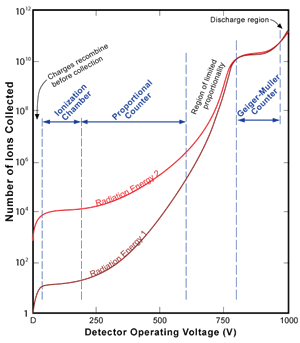
\includegraphics[scale=0.9]{img/detectorvoltage.png}
  \caption{detectorvoltage}
  \label{fig:detectorvoltage}
\end{figure}
Quelle: \url{https://www.nde-ed.org/index_flash.htm}
\subsubsection{Taschen-Dosimeter}
Pocket-Dosimeter werden verwendet, um dem Träger eine sofortige Ablesung seiner Exposition gegenüber Röntgen- und Gammastrahlen zu ermöglichen. Wie der Name schon sagt, werden sie häufig in der Tasche getragen. Die beiden in der industriellen Radiographie gebräuchlichen Typen sind das Direct Read Pocket Dosimeter und das Digital Electronic Dosimeter.
\subsubsection{Direct Read Pocket Dosimeter}
Ein direkt lesendes Taschenionisationsdosimeter hat im Allgemeinen die Größe und Form eines Füllhalters. Das Dosimeter enthält eine kleine Ionisationskammer mit einem Volumen von ungefähr zwei Millilitern. In der Ionisationskammer befindet sich eine zentrale Drahtanode, und an dieser Drahtanode ist eine metallbeschichtete Quarzfaser befestigt. Wenn die Anode auf ein positives Potential geladen ist, wird die Ladung zwischen der Drahtanode und der Quarzfaser verteilt. Elektrostatische Abstoßung lenkt die Quarzfaser ab, und je größer die Ladung ist, desto größer ist die Ablenkung der Quarzfaser. Strahlung, die auf die Kammer einfällt, erzeugt eine Ionisierung innerhalb des aktiven Volumens der Kammer. Die durch Ionisation erzeugten Elektronen werden von der positiv geladenen zentralen Anode angezogen und gesammelt. Diese Ansammlung von Elektronen reduziert die positive Nettoladung und ermöglicht, dass die Quarzfaser in Richtung der ursprünglichen Position zurückkehrt. Die Menge der Bewegung ist direkt proportional zu der Menge der Ionisation, die auftritt.\\
\begin{figure}[htb]
  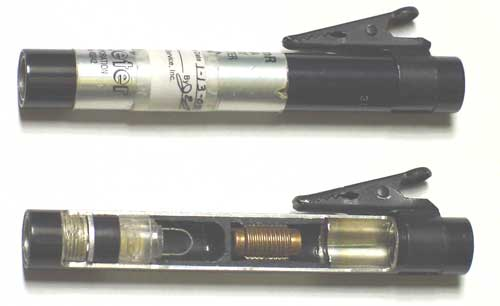
\includegraphics[scale=0.3]{img/dosimeter&cutaway.jpg}\\
  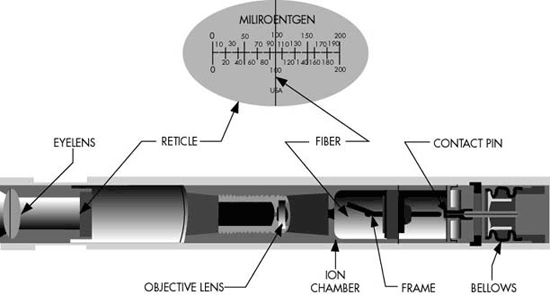
\includegraphics[scale=0.3]{img/dose.png}
  \caption{Pocket-Dosimeter}
  \label{fig:Pocket-Dosimeter}
  Quelle: \url{https://www.nde-ed.org/index_flash.htm}
\end{figure}\\


Indem das Instrument auf eine Lichtquelle gerichtet wird, kann die Position der Faser durch ein System von eingebauten Linsen beobachtet werden. Die Faser wird auf einer lichtdurchlässigen Skala betrachtet, die in Belichtungseinheiten abgestuft ist. Typische industrielle Röntgendiagnostik-Taschen-Dosimeter haben eine volle Skala von 200 Milliröntgen, aber es gibt Designs, die höhere Mengen aufzeichnen werden. Während der Schicht sollte der Dosimeterstand häufig überprüft werden. Die gemessene Exposition sollte am Ende jeder Schicht aufgezeichnet werden.
Der Hauptvorteil eines Taschendosimeters besteht in seiner Fähigkeit, dem Träger eine sofortige Ablesung seiner Strahlenbelastung zu ermöglichen. Es hat auch den Vorteil, wiederverwendbar zu sein. Die begrenzte Reichweite, die Unfähigkeit, eine dauerhafte Aufzeichnung zu liefern, und das Potenzial für Entlade- und Leseverluste aufgrund von Stürzen oder Stoßen sind einige der Hauptnachteile eines Taschendosimeters. Die Dosimeter müssen zu Beginn jeder Arbeitsschicht aufgeladen und aufgezeichnet werden. Ladungsverlust oder -drift können ebenfalls das Ablesen eines Dosimeters beeinflussen. Die Leckage sollte in einem Zeitraum von 24 Stunden nicht mehr als 2 Prozent des vollen Skalenwerts betragen.
\subsubsection{Digitales elektronisches Dosimeter}
Eine andere Art von Dosimeter ist das digitale Dosimeter. Diese Dosimeter zeichnen Dosisinformation und Dosisrate auf. Diese Dosimeter verwenden meistens Geiger-Müller-Zähler. Die Ausgabe des Strahlungsdetektors wird gesammelt, und wenn eine vorbestimmte Belichtung erreicht worden ist, wird die gesammelte Ladung entladen, um einen elektronischen Zähler auszulösen.
Der Zähler zeigt dann die akkumulierte Belichtung und Dosisrate in digitaler Form an.
Einige digitale elektronische Dosimeter enthalten eine akustische Alarmfunktion, die bei jeder aufgenommenen Belichtungsstufe ein akustisches Signal oder einen Piepton ausgibt. Einige Modelle können auch so eingestellt werden, dass ein kontinuierliches akustisches Signal ertönt, wenn eine voreingestellte Belichtung erreicht wurde. Dieses Format hilft, die Lesefehler zu minimieren, die mit direkt lesenden Taschenionisationskammer-Dosimetern verbunden sind, und ermöglicht es dem Instrument, eine höhere maximale Auslesung zu erreichen, bevor das Rücksetzen notwendig ist.
\begin{figure}[htb]
\centering
  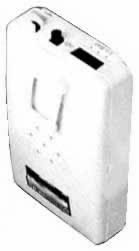
\includegraphics[scale=0.3]{img/Digital-Dosimeter.jpg}\\
  \caption{Pocket-Dosimeter}
  \label{fig:Pocket-Dosimeter}
  Quelle: \url{https://www.nde-ed.org/index_flash.htm}
\end{figure}
\subsubsection{Akustische Alarmgeräte-Meter und digitale elektronische Dosimeter}
Akustische Alarme sind Geräte, die einen kurzen Piep abgeben, wenn eine vorbestimmte Belichtung empfangen wurde.
Es ist erforderlich, dass diese elektronischen Geräte von Personen getragen werden, die mit Gammastrahlern arbeiten. Diese Vorrichtungen verringern die Wahrscheinlichkeit von zufälligen Aussetzungen in der industriellen Radiographie, indem sie den Radiographen auf Strahlendosen oberhalb einer voreingestellten Menge warnen. Typische Alarmratenmessgeräte beginnen in Bereichen von 450-500 mR / h zu erklingen. Es ist wichtig zu beachten, dass akustische Alarme nicht dazu gedacht sind und nicht als Ersatz für Vermessungsmesser verwendet werden sollten.\\
Die meisten akustischen Alarme verwenden einen Geiger-Müller-Detektor. Die Ausgabe des Detektors wird gesammelt, und wenn eine vorbestimmte Belichtung erreicht worden ist, wird diese gesammelte Ladung durch einen Lautsprecher entladen. Daher wird ein hörbarer Piep abgegeben. Folglich ist die Frequenz oder die Chirp-Rate des Alarms proportional zur Strahlungsintensität. Die Chirp-Rate variiert zwischen verschiedenen Alarmen von einem Chirp pro Milliröntgen bis zu mehr als 100 Chirps pro Milliröntgen.
\begin{figure}[htb]
\centering
   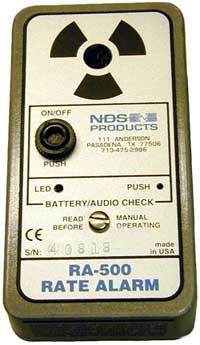
\includegraphics[scale=0.3]{img/alarm.jpg}\\
  \caption{Akustische Alarmgeräte}
  \label{fig:Alarmgeräte Meter}
  Quelle: \url{https://www.nde-ed.org/index_flash.htm}
\end{figure}
\subsubsection{Film Badges}
Personendosimetrie-Filmabzeichen werden üblicherweise verwendet, um die Strahlenbelastung aufgrund von Gammastrahlen, Röntgenstrahlen und Betateilchen zu messen und aufzuzeichnen. Der Detektor ist, wie der Name schon sagt, ein Stück strahlungsempfindlichen Film. Die Folie ist in einer lichtdichten, dampfdichten Hülle verpackt, die verhindert, dass Licht, Feuchtigkeit oder chemische Dämpfe auf den Film einwirken.
\begin{figure}[htb]
   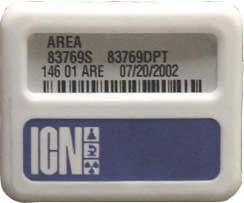
\includegraphics[scale=0.7]{img/area-filmbadge.jpg}\\
   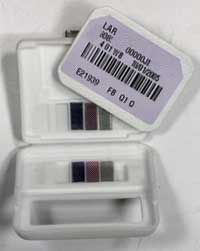
\includegraphics[scale=0.5]{img/FilmBadge.jpg}\\
  \caption{FilmBadge}
  \label{fig:FilmBadge}
  Quelle: \url{https://www.nde-ed.org/index_flash.htm}
\end{figure}
Es wird ein spezieller Film verwendet, der mit zwei verschiedenen Emulsionen beschichtet ist. Eine Seite ist mit einer großkörnigen, schnellen Emulsion beschichtet, die empfindlich auf geringe Expositionen reagiert. Die andere Seite des Films ist mit einer feinkörnigen, langsamen Emulsion beschichtet, die weniger empfindlich gegenüber Belichtung ist. Wenn die Strahlenexposition dazu führt, dass die schnelle Emulsion in dem verarbeiteten Film zu einem Grad verdunkelt wird, der nicht interpretiert werden kann, wird die schnelle Emulsion entfernt und die Dosis wird unter Verwendung der langsamen Emulsion berechnet.
Der Film ist in einem Filmhalter oder Abzeichen enthalten. Das Abzeichen enthält eine Reihe von Filtern, um die Qualität der Strahlung zu bestimmen. Die Strahlung einer gegebenen Energie wird in unterschiedlichem Maße durch verschiedene Arten von Absorbern abgeschwächt. Daher wird die gleiche Strahlungsmenge, die auf die Plakette auftrifft, unter jedem Filter einen unterschiedlichen Grad an Dunkelfärbung erzeugen. Durch Vergleich dieser Ergebnisse kann die Energie der Strahlung bestimmt und die Dosis berechnet werden, wobei die Filmantwort für diese Energie bekannt ist. Der Ausweishalter enthält außerdem ein offenes Fenster zur Bestimmung der Strahlenbelastung durch Betateilchen. Betateilchen werden effektiv durch eine geringe Menge an Material abgeschirmt.
Die Hauptvorteile eines Filmabzeichens als Personalüberwachungsgerät sind, dass es eine dauerhafte Aufzeichnung bereitstellt, es in der Lage ist, zwischen verschiedenen Energien von Photonen zu unterscheiden, und es Dosen aufgrund verschiedener Arten von Strahlung messen kann. Es ist ziemlich genau für Belichtungen größer als 100 Millirem. 
Die Hauptnachteile bestehen darin, dass sie von einem Prozessor entwickelt und gelesen werden müssen (was zeitaufwendig ist), eine längere Hitzeeinwirkung den Film beeinträchtigen kann und Belichtungen von weniger als 20 Milliram Gammastrahlung nicht genau gemessen werden können.
Filmabzeichen müssen korrekt getragen werden, damit die Dosis, die sie erhalten, genau die Dosis darstellt, die der Träger erhält. Ganzkörper-Abzeichen werden am Körper zwischen Hals und Taille getragen, oft am Gürtel oder an der Hemdtasche. Das Ansteck-Abzeichen wird am häufigsten bei der Röntgen- oder Gammaradiographie getragen. Das Filmabzeichen kann auch beim Arbeiten in einer niedrigen Curie-Quelle getragen werden. Ringabzeichen werden an einem Finger der Hand getragen, der am wahrscheinlichsten ionisierender Strahlung ausgesetzt ist. Ein LIXI-System mit seinem kulminierten und gerichteten Strahl wäre ein Beispiel, bei dem die Überwachung der Hände wichtiger wäre als der gesamte Körper.
\subsubsection{Thermoluminescent Dosimeter (TLD)}
Thermoluminescent Dosimeter(TLD) werden oft anstelle des Filmabzeichens verwendet. Wie ein Filmabzeichen wird es für eine gewisse Zeit (normalerweise 3 Monate oder weniger) getragen und muss dann verarbeitet werden, um die erhaltene Dosis zu bestimmen, falls vorhanden. Thermoluminescent Dosimeter können Dosierungen bis zu 1 Millirem messen, aber unter Routinebedingungen ist ihre niedrige Dosisleistung ungefähr die gleiche wie für Filmabzeichen. TLDs haben eine Genauigkeit von ca. 15\% für niedrige Dosen. Diese Genauigkeit verbessert sich bei hohen Dosen auf etwa 3\%. Die Vorteile einer TLD gegenüber anderen Personalmonitoren sind ihre Linearität der Reaktion auf die Dosis, ihre relative Energieunabhängigkeit und ihre Empfindlichkeit gegenüber niedrigen Dosen. Es ist auch wiederverwendbar, was ein Vorteil gegenüber Filmabzeichen ist. Es wird jedoch keine dauerhafte Aufzeichnung oder Wiederlesbarkeit bereitgestellt, und eine sofortige Auslesung am Arbeitsplatz ist nicht möglich.
\begin{figure}[htb]
\centering
   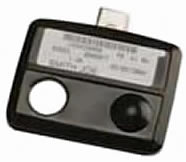
\includegraphics[scale=0.9]{img/TLD.jpg}\\
  \caption{TLD}
  \label{fig:TLD}
  Quelle: \url{https://www.nde-ed.org/index_flash.htm}
\end{figure}
\subsubsection{Wie es funktioniert}
Eine TLD ist ein Phosphor, wie Lithiumfluorid (LiF) oder Calciumfluorid (CaF), in einer festen Kristallstruktur. Wenn eine TLD ionisierende Strahlung bei Umgebungstemperaturen ausgesetzt wird, wechselwirkt die Strahlung mit dem Phosphorkristall und deponiert die gesamte oder einen Teil der einfallenden Energie in diesem Material. Einige der Atome im Material, die diese Energie absorbieren, werden ionisiert und erzeugen freie Elektronen und Bereiche, denen ein oder mehrere Elektronen fehlen, Löcher genannt. Unvollkommenheiten in der Kristallgitterstruktur wirken als Stellen, an denen freie Elektronen eingeschlossen und an Ort und Stelle arretiert werden können.
Durch Erhitzen des Kristalls vibriert das Kristallgitter, wodurch die eingefangenen Elektronen freigesetzt werden. Freigesetzte Elektronen kehren in den ursprünglichen Grundzustand zurück und geben die eingefangene Energie aus der Ionisation als Licht frei, daher der Name Thermolumineszenz. Freigesetztes Licht wird unter Verwendung von Photovervielfacherröhren gezählt, und die Anzahl der gezählten Photonen ist proportional zu der Strahlungsmenge, die auf den Phosphor trifft.
Anstatt die optische Dichte (Schwärze) eines Films zu lesen, wie es bei Filmabzeichen der Fall ist, wird die Menge an Licht gemessen, die gegenüber dem Erwärmen der einzelnen Stücke des Thermolumineszenzmaterials freigesetzt wird. Die durch diesen Prozess erzeugte TLD-Kurve steht dann in Beziehung zur Strahlenbelastung. Der Prozess kann viele Male wiederholt werden.

























































